%!TEX root = ../3dbook.tex
% chktex-file 18 
% chktex-file 46

\setchapterpreamble[u]{\margintoc}

\graphicspath{{3dcm/}}
% \renewcommand*{\thelesson}{4.1}

\chapter{Semantic 3D city models}%
\label{chap:3dcm}

A 3D city model is a digital representation,  with three-dimensional geometries, of the common objects in an urban environment, with buildings usually being the most prominent objects. 

Because typical 3D city models are reconstructed/derived from various acquisition techniques, their structure, format, and characteristic will greatly vary.
As an example, a 3D city model can be reconstructed with methods such as these: photogrammetry, laser scanning, extrusion from 2D footprints, conversion from architectural models and drawings, procedural modelling, volunteered geoinformation, etc.

This chapter discusses the main 3D city models formats, and focuses on \emph{semantic} 3D city models, 
\marginnote{semantic 3D city models}\index{semantics}
which are useful in a variety of applications.


%%%
%
\section{Semantic 3D city models}

Consider the 3D city model of Helsinki in Figure~\ref{fig:mesh}a (one part of it),
\begin{figure*}
  \centering
  \begin{subfigure}[b]{0.48\linewidth}
    \centering
    \includegraphics[width=\textwidth]{figs/mesh01.png}
    \caption{}
  \end{subfigure}
  \begin{subfigure}[b]{0.48\linewidth}
    \centering
    \includegraphics[width=\textwidth]{figs/mesh04.png}
    \caption{the edges of the triangles are highlighted in orange.}
  \end{subfigure}
\caption{Part of the 3D city model of Helsinki, Finland.}%
\label{fig:mesh}
\end{figure*}
which was reconstructed by dense matching of aerial images.
The model is a textured mesh, formed by triangles to which a texture is attached (the triangles are visible in Figure~\ref{fig:mesh}b).
\marginnote{textured mesh}\index{textured mesh}
If you were asked to count the number of buildings (or cars, or dormers in a given building) you would surely just have to zoom in on the model, look at it, and then you could give the answer.
However, for a computer, this 3D city model is simply represented as a series of triangles to which a texture is attached; the notion of `building' (or `car', or any other object) is thus not available.
As a result, a computer cannot automatically answer these simple questions.
It should be observed that there exist algorithms to segment and classify textured meshes into objects, but these are not fully automatic (yet!) and are beyond the scope of this book.
Other simple questions that a human could easily answer but a computer cannot:
\begin{enumerate}
  \item how many windows does the main façade of a given building have?
  \item how many floors does a given building have?
  \item can the local park be seen from the second floor of a given building?
\end{enumerate}

%

A semantic 3D city model is a data model where the \emph{relevant} objects (and their sub-parts) are labelled with their meaning and have attributes attached to them.
Conceptually, it means that a city is decomposed 
\marginnote{decomposition of a city into relevant classes}
into classes that we deem relevant for certain applications, for instance the city is decomposed into the classes `building', `road', `tree', `lamppost', etc, and each of the objects has its own 3D geometry and potentially (thematic) attributes (\eg\ the owner of a building, the name of street, the city identifier for a lamppost, etc).

%

Observe also, as shown in Figure~\ref{fig:ssc} for one building, 
\begin{figure*}
  \centering
  \includegraphics[width=\linewidth]{figs/ssc}
  \caption[A building is semantically decomposed into different objects]{A building is semantically decomposed into different objects, and each objects is defined with geometry. This building has good spatio-semantic coherence}%
\label{fig:ssc}
\end{figure*}
that the objects can be further decomposed into semantically homogeneous parts, in 3D city modelling these are often the parts of a buildings (\eg\ an extension to a house) and the type of surfaces (roof, façade, window, door).

The decomposition is thus \emph{hierarchical}, 
\marginnote{hierarchical decomposition}
and the relationships between the classes are stored (\eg\ a building is composed of parts, which are formed of walls/grounds/roofs, which have windows). 
We say that a 3D city model is \emph{spatio-semantically coherent} if the two decompositions are coherent,
\marginnote{spatio-semantic coherence}\index{spatio-semantic coherence}
that is if there is a one-to-one mapping between the elements of each decomposition (geometry and semantic), see Figure~\ref{fig:ssc} for one example.
% containing two parts, would be decomposed semantically and geometrically; notice that both decompositions should ideally be coherent.
% but parts of those (roof and façade surfaces, dormers, side-walks))

%

Figure~\ref{fig:denhaag} shows one semantic model being visualised in a viewer, notice that the user can identify the roof surfaces and that different attributes are available.
\begin{figure*}
  \centering
  \includegraphics[width=\linewidth]{figs/denhaag.jpg}
  \caption[Part of the semantic 3D city model of The Hague]{Part of the semantic 3D city model of The Hague, in the Netherlands. Notice that each building is decomposed into its semantic surfaces (wall, roof, and ground) and there are attributes for each. The model is not textured, but semantic models can have textures too.}%
\label{fig:denhaag}
\end{figure*}

%

It should also be noticed that semantic 3D models can be textured.

%

To avoid the fact that every city/country defines its own classes to decompose a city (\eg\ a `building' class can be a `house' class in another city), semantic models prescribe the classes and often even the thematic attributes that should be stored.


% TODO: add this somewhere?
% The CityGML data model defines ways to describe most of the common 3D features and objects found in cities and the relationships between them. 
% These can be supplemented with textures and/or colours to give a better impression of their appearance.
% Specific relationships between different objects can also be stored using CityGML, for example that a building is decomposed into three parts, or that a building has a both a carport and a balcony.


%%%
%
\section[CityGML data model]{The CityGML data model}%
\index{CityJSON}

CityGML is an open data model to represent semantic 3D models of cities and landscapes, and it is standardised by the Open Geospatial Consortium (OGC). 
\marginnote{\faExternalLink\ \url{https://www.opengeospatial.org/standards/citygml}}
Its first version (v1.0.0) was released in 2008, and the current version (v3.0.0) in 2021.

The classes possible in CityGML are grouped into different modules, as can be seen in Figure~\ref{fig:citygml_modules}.
\begin{marginfigure}
  \centering
  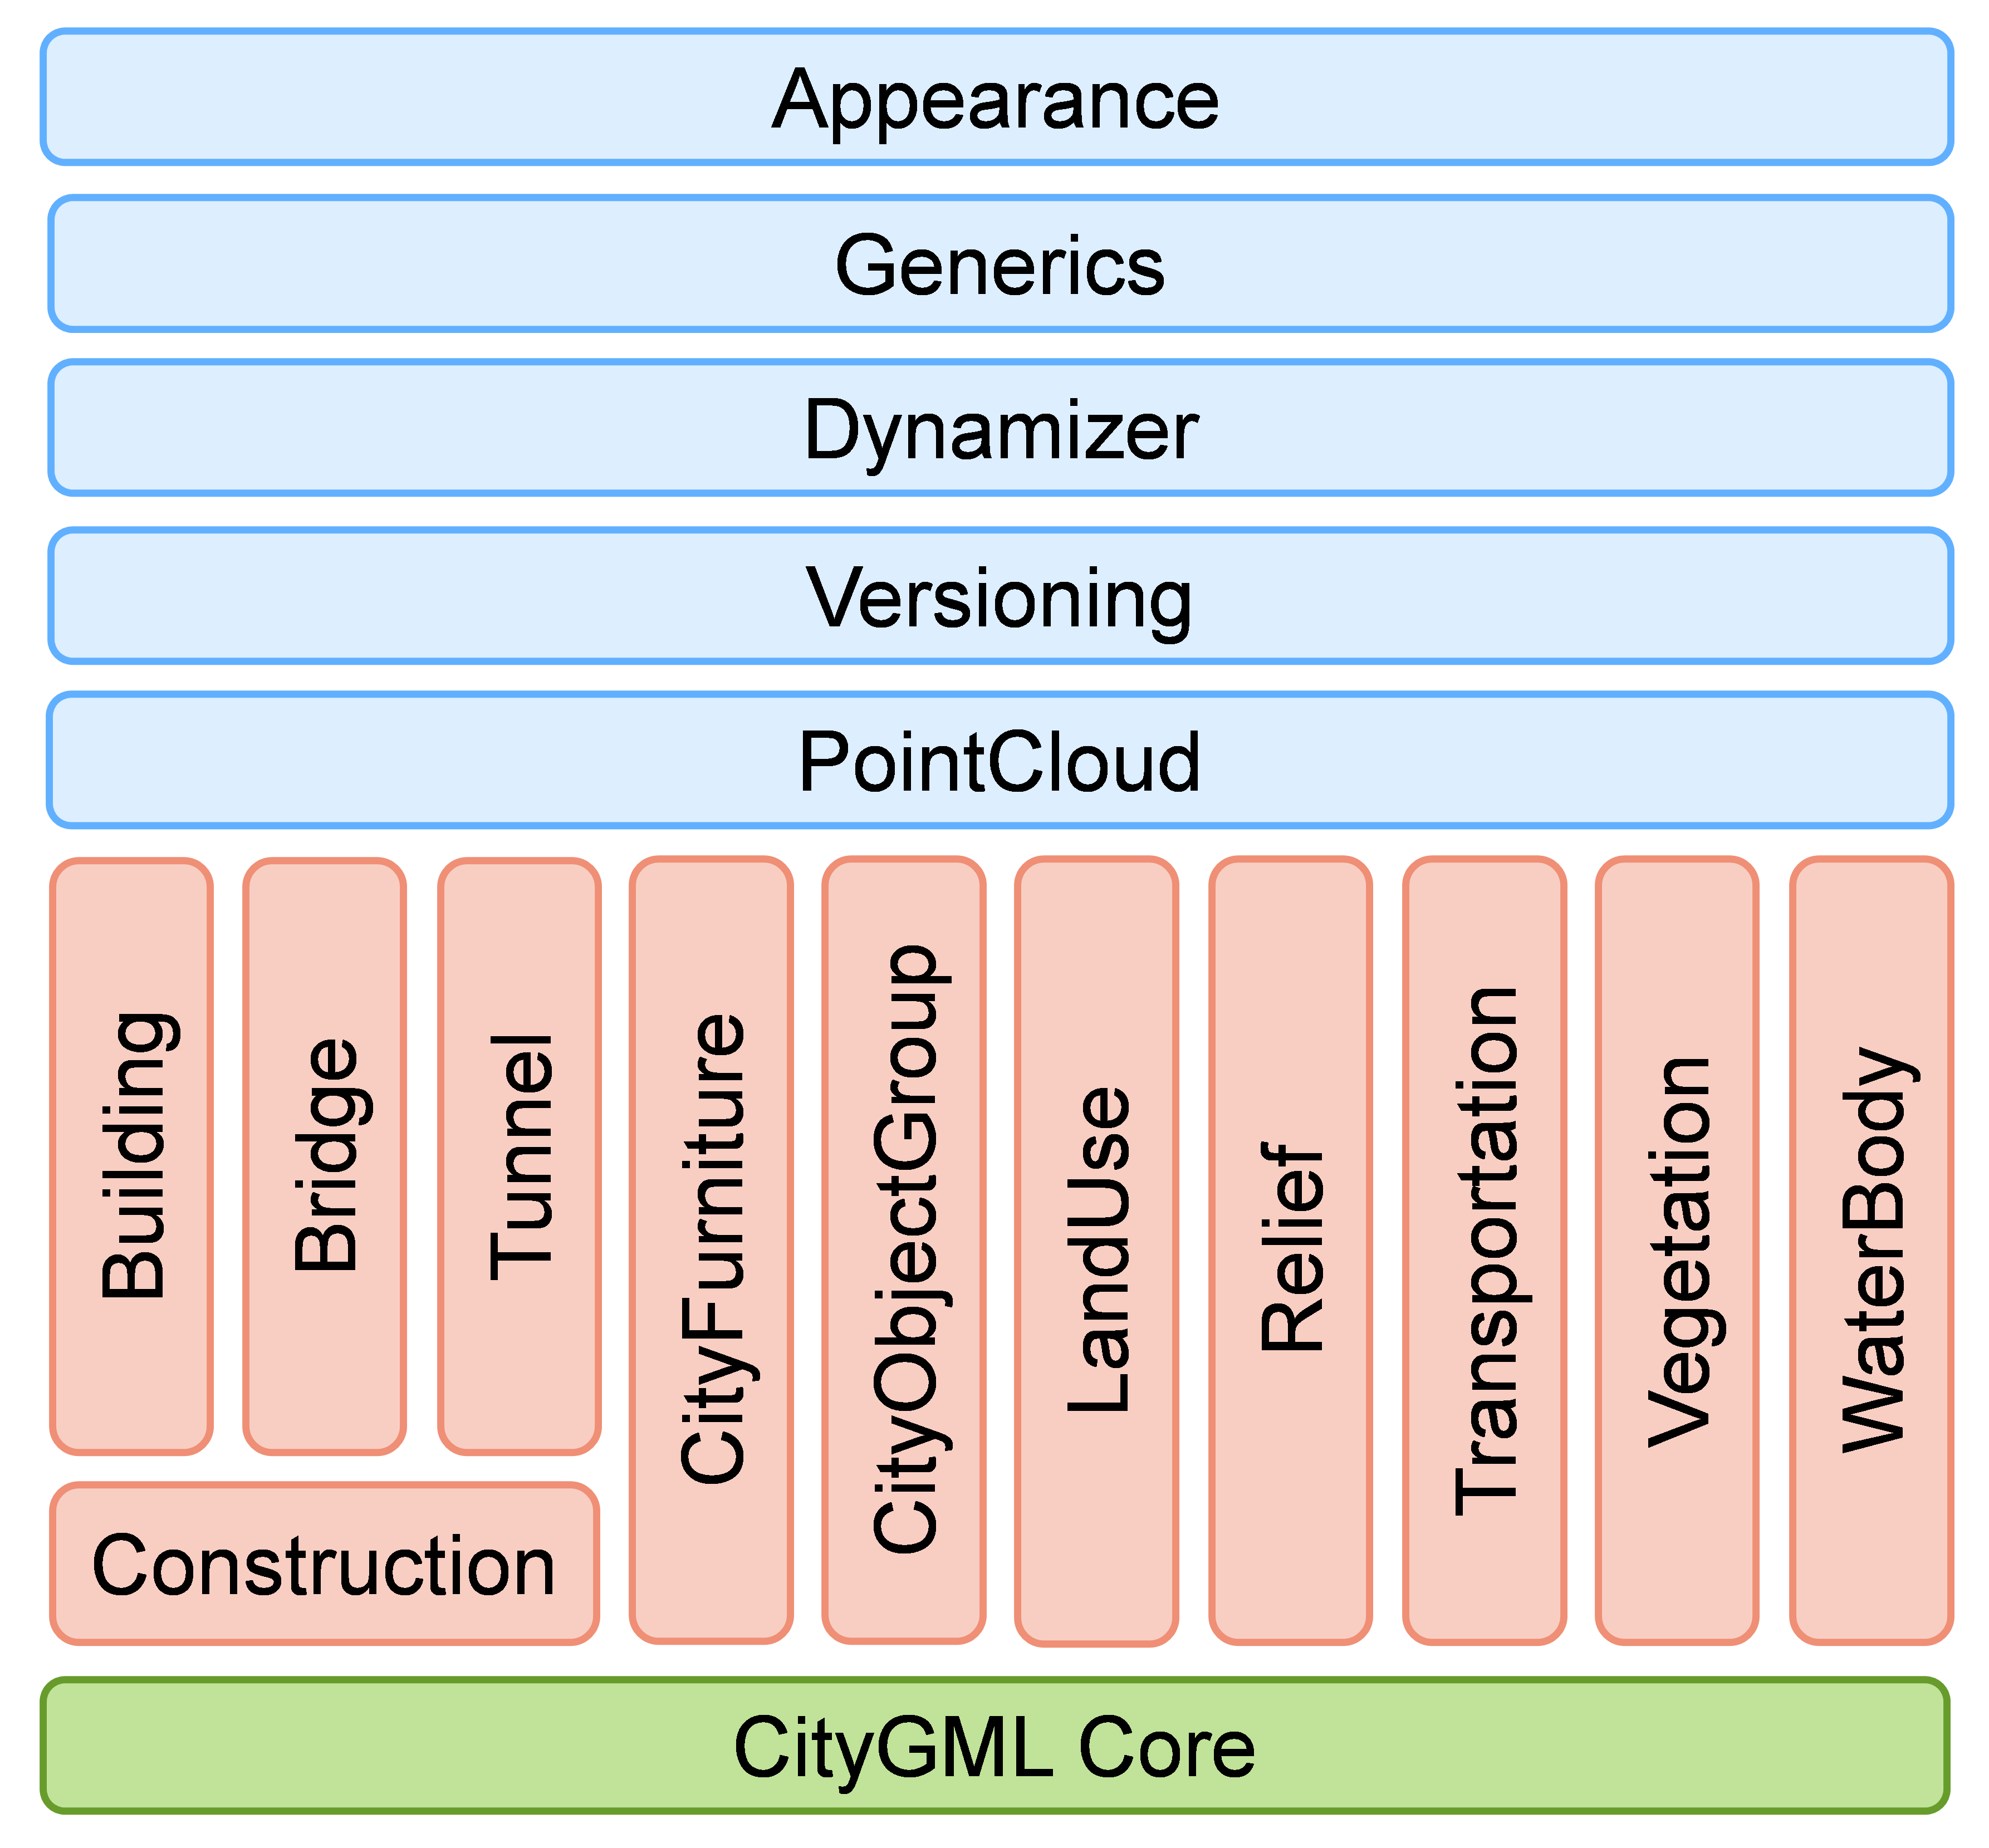
\includegraphics[width=\linewidth]{figs/citygml_modules.png}
  \caption{The modules of the CityGML data model.}%
\label{fig:citygml_modules}
\end{marginfigure}
In the specifications, each module is described with text and the UML diagram of the classes is available.
Figure~\ref{fig:citygml_uml_core} shows the core module, and Figure~\ref{fig:citygml_uml_building} the classes for the Building module.
It can be seen that both the exterior and the interior of a building can be described, a building can for instance have different rooms (\emph{BuildingRoom}), different storeys or units (\texttt{BuildingStorey} and \texttt{BuildingUnit}), but also installations (\eg\ chimneys, antennas, balconies, etc.).
\begin{figure*}
  \centering
  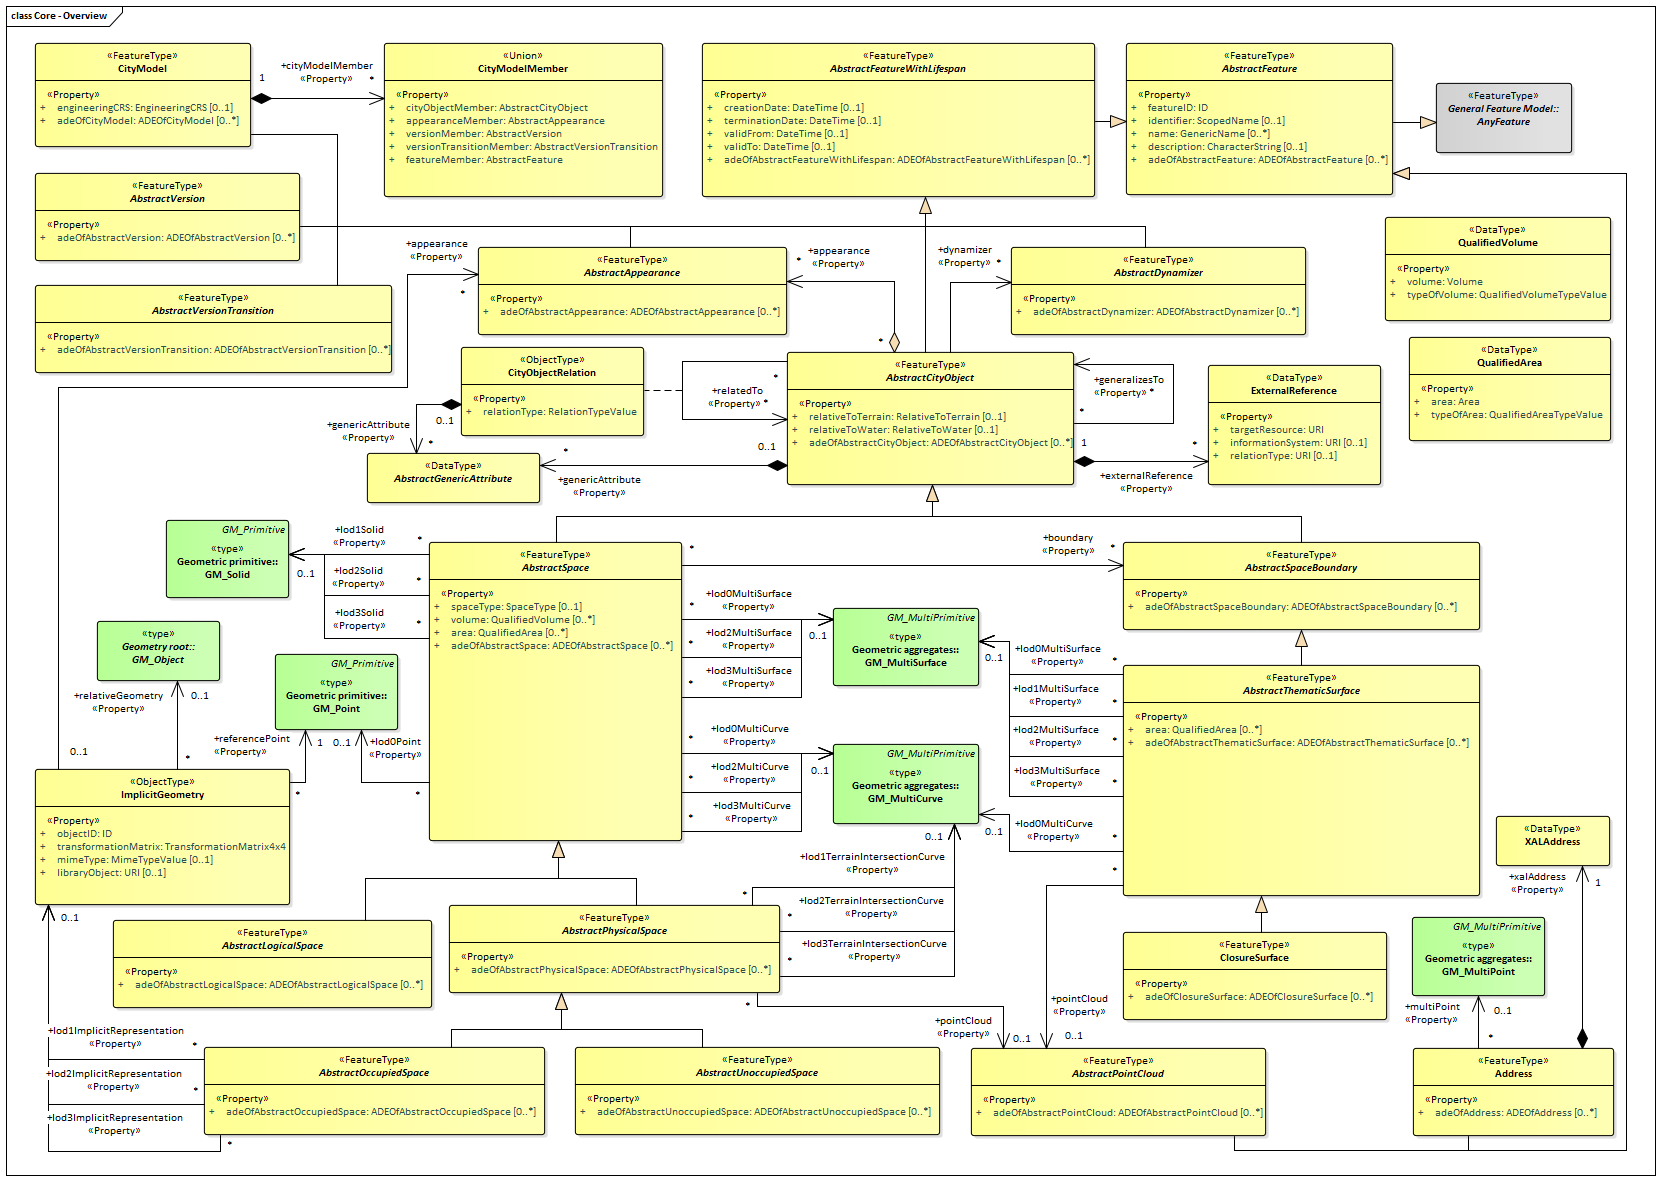
\includegraphics[width=0.95\linewidth]{figs/citygml_uml_core}
  \caption[Overview of the UML model for the core of CityGML]{Overview of the UML model for the core of CityGML\@. (Figure \textcopyright\ 2021 Open Geospatial Consortium, Inc.)}%
\label{fig:citygml_uml_core}
\end{figure*}
\begin{figure*}
  \centering
  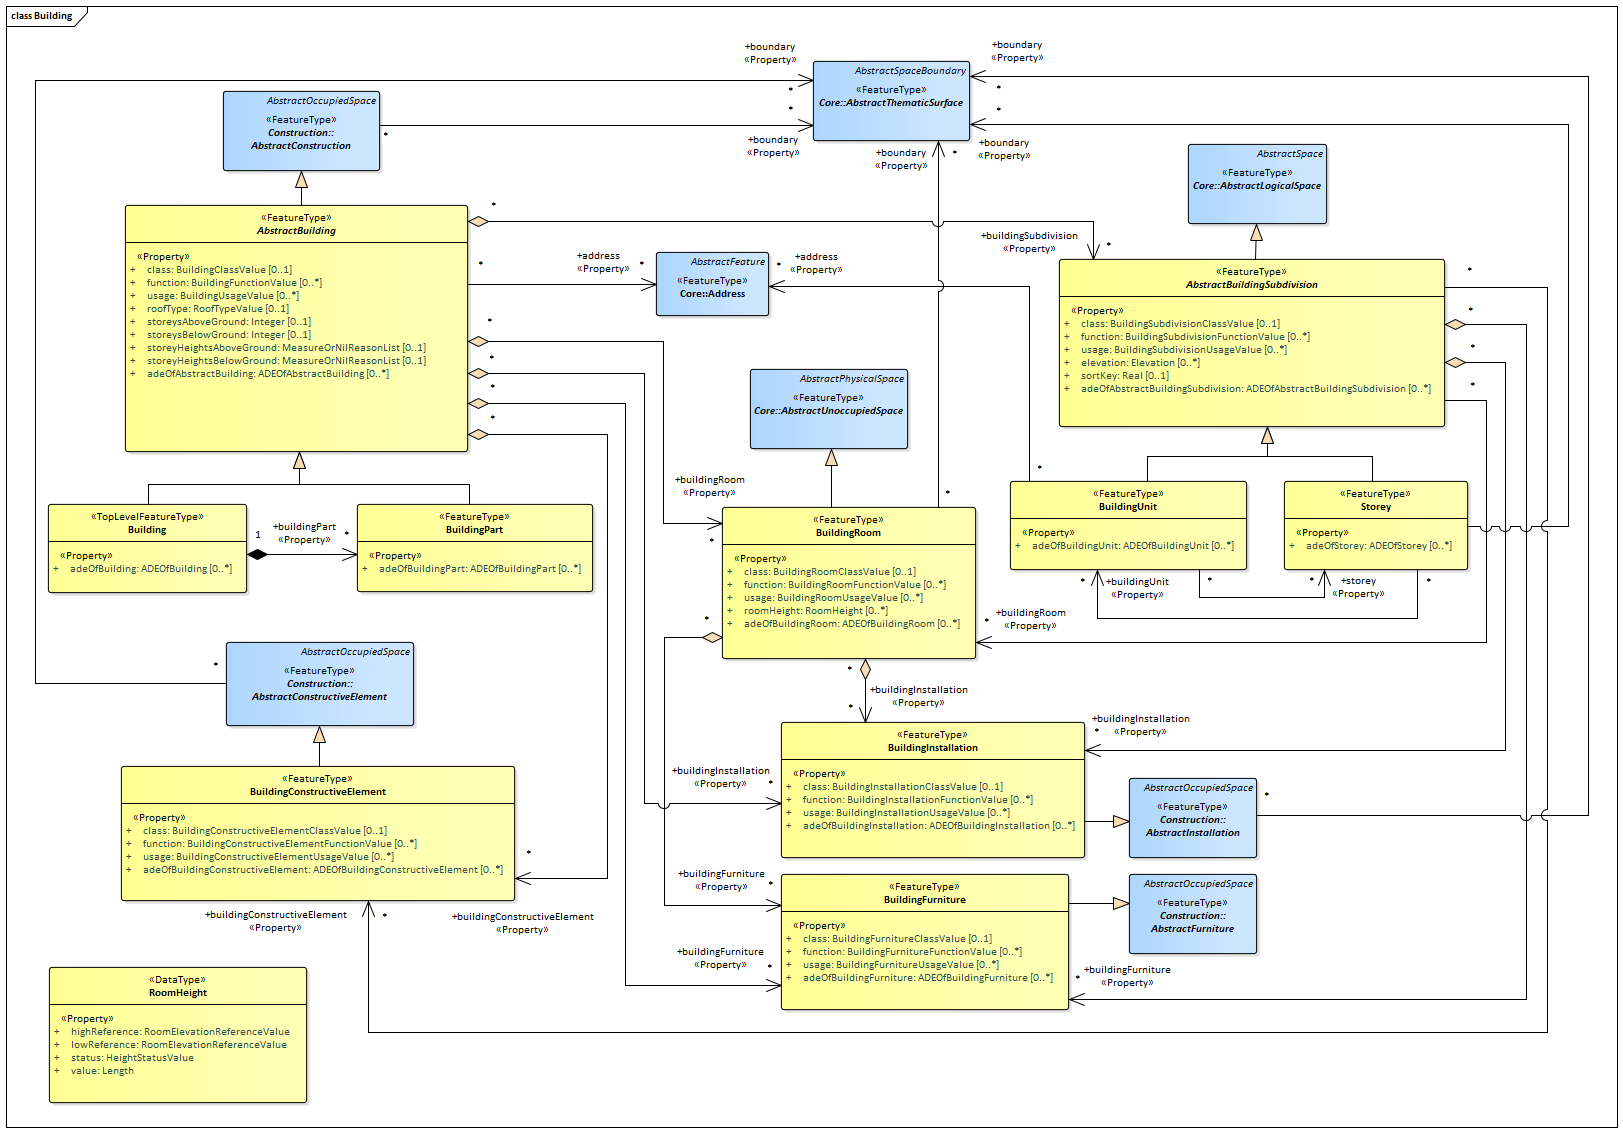
\includegraphics[width=0.95\linewidth]{figs/citygml_uml_building}
  \caption[Overview of the UML model for the core of CityGML]{Overview of the UML model for the core of CityGML\@. (Figure \textcopyright\ 2021 Open Geospatial Consortium, Inc.)}%
\label{fig:citygml_uml_building}
\end{figure*}



%

\subsection{Levels-of-detail (LoDs)}%
\label{sec:lods}

One particularity of CityGML is that it prescribes the different standard levels of detail (LoDs) for 3D objects, which allows us to represent objects for different applications and purposes.

For each of the modules defined by CityGML, four LoDs can be defined.
Figure~\ref{fig:officiallods}
\begin{marginfigure}
  \centering
  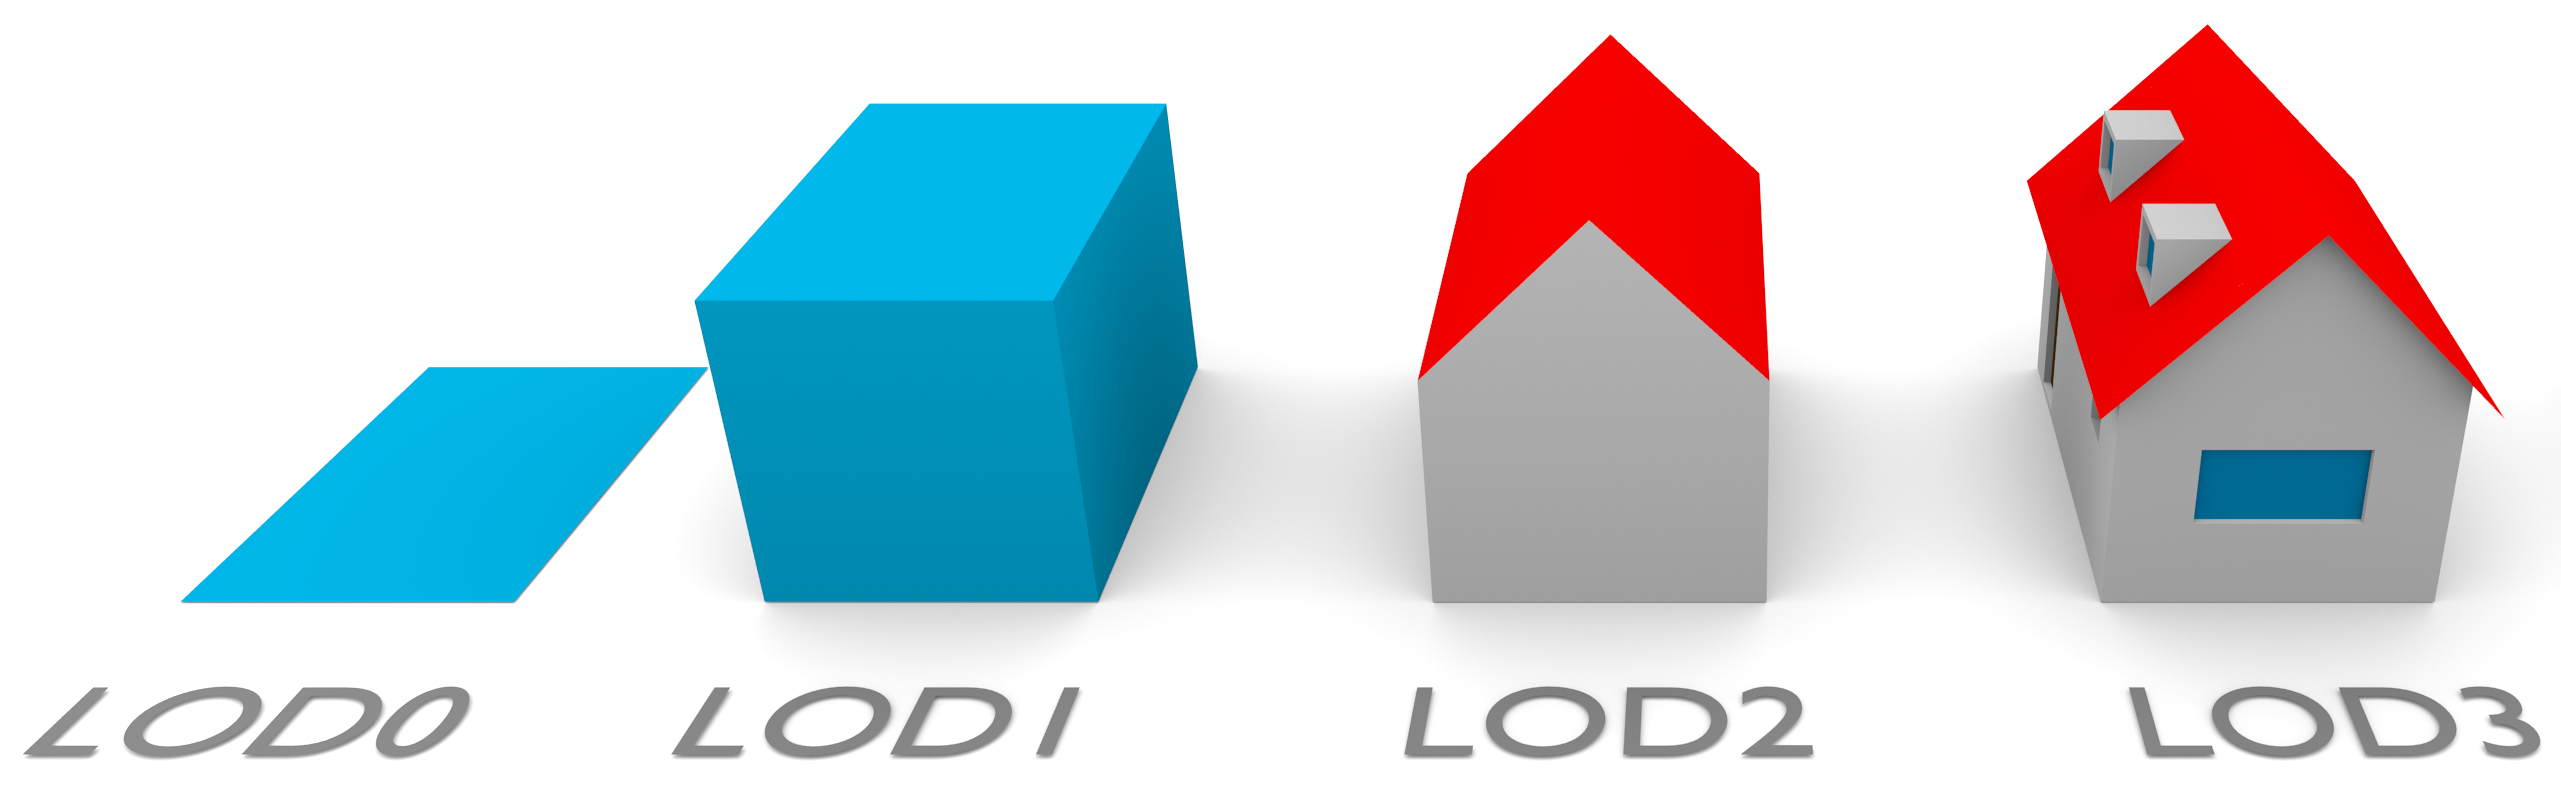
\includegraphics[width=\textwidth]{figs/CityGML-LODs-c3.png}
  \caption{The four LoDs in CityGML for the exterior of a building.}%
\label{fig:officiallods}
\end{marginfigure}
shows the ones for the buildings, and they are as follows:
\begin{description}
  \item[LoD0] is a horizontal polygon representing the footprint (at the elevation of the terrain) and optionally a horizontal polygon representing the horizontal roof.
  Such models represent the transition from 2D to 3D GIS, and they do not contain volumetric geometries.
  \item[LoD1] is a block model, with an horizontal and planar roof that is usually derived by extruding a footprint to a given height.
  LoD1 models are easy to reconstruct: the footprint of a building, readily available in many countries, can be extruded to its height. The height can be the average (or median) of all the lidar points inside the footprint.
  \item[LoD2] the generalised roof shape and larger roof superstructures are present.
  As such, LoD2 models are useful for rooftop solar potential estimations.
  They are usually obtained with photogrammetric techniques, and, in some cases, may be derived automatically (see Chapter~\ref{chap:LoD2recon}). 
  \item[LoD3] is a detailed architectural model containing openings (windows and doors), chimneys, and other façade details.
  Models at LoD3 are usually obtained with a conversion from BIM models or from terrestrial laser scanning.
  The presence of windows and other details makes them useful in applications such as energy simulations.
\end{description}

%

The interior of a building can also be modelled by using the following classes: \texttt{BuildingStorey}, \texttt{BuildingRoom}, or \texttt{BuildingUnit}.
For each of these, it is possible to use one of the LoD (from LoD0 to LoD3), although the details have not be standardised.
  \begin{marginfigure}
    \centering
    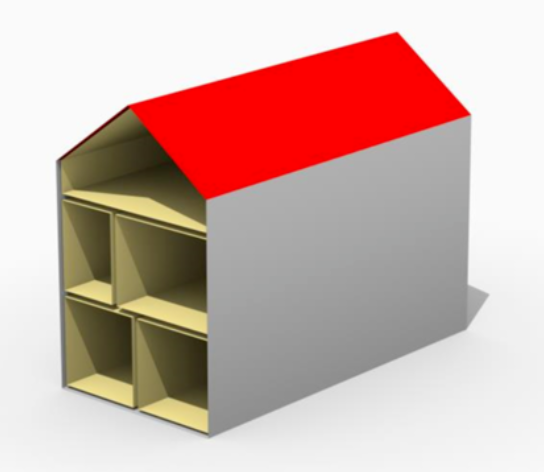
\includegraphics[width=\linewidth]{figs/lod4}
    \caption[The subdivision of the interior of a building can be modelled]{The subdivision of the interior of a building can be modelled. Figure from \citet{Lowner16}}%
  \label{fig:lod4}
  \end{marginfigure}
We usually assume that lower LoDs have less geometrical and semantical details than higher ones.

%

While the four LoDs are supposed to inform users about the representation of the data, in practice they are too generic (not precise enough) and can be ambiguous. 
For instance, as Figure~\ref{fig:lod_ambiguity} shows,
\begin{marginfigure}
  \centering
  \includegraphics[width=\linewidth]{figs/lod_ambiguity_b}
  \caption[Two buildings represented in CityGML as LoD2 models]{Two buildings represented in CityGML as LoD2 models. Both are valid LoD2 models.}%
\label{fig:lod_ambiguity}
\end{marginfigure}
a building with roof overhangs can be modelled as LoD2 with them, or without (and therefore the size of its footprint would be larger).
Both are technically ``valid'' LoD2 models, but the acquisition methods required differ significantly.
The model on the right can be acquired with aerial photogrammetry or aerial lidar (the walls are derived as projections from the roof outline), while the model on the left probably needs two acquisition techniques: the walls are at their actual location (ground survey was necessary) and the roof overhangs are explicitly present.
To remedy to this situation, improved LoDs for buildings have been proposed at TU Delft, see Figure~\ref{fig:refinedLODs}.
\begin{figure}
  \centering
  \includegraphics[width=0.9\linewidth]{figs/refinedLODs}
  \caption[The TUDelft LoDs]{The improved LoDs for buildings; they are generally referred to as the \emph{TUDelft LoDs}.}%
\label{fig:refinedLODs}
\end{figure}

%

Notice that while each of the CityGML classes can be represented with four different LoDs, only those for buildings are prescribed and documented.
For trees and roads, practitioners can decide that a given representation is `LoD2', 
\marginnote{LoDs for trees and roads}
but that would purely indicate that the LoD is higher than a LoD1 one.
There are efforts (scientific papers) to document these, but they have not been standardised (yet).


%%%
\subsection{Geometries}

CityGML uses the ISO19107 geometric primitives for representing the geometry of its 3D objects.
\marginnote{ISO19107 is used, with a few restrictions}\index{ISO19107}
While the ISO19107 primitives do not need to be linear or planar, \ie\ curves defined by mathematical functions are allowed, CityGML uses a subset of ISO19107, with the following two restrictions: (1) \texttt{GM\_Curves} can only be \emph{linear} (thus only \texttt{LineStrings} and \texttt{LinearRings} are used); (2) \texttt{GM\_Surfaces} can only be \emph{planar} (thus \texttt{Polygons} are used).

See Chapter~\ref{chap:iso19107} for ISO19107.


%%%
\subsection{Textures and materials}
The 3D geometries can be supplemented with textures and/or colours (called materials since different parameters like transparency can be defined) to give a better impression of their appearance.

CityGML reuses known and used standards in other fields for the appearances.
The material is represented with the X3D specifications, and the texture with the COLLADA standard.


%%%
\subsection{Extensions to the core data model with ADEs} 

The CityGML data model prescribes a certain number of classes, but sometimes practitioners may want to model additional objects.
For this, CityGML has the concept of ADEs (application domain extensions).
\marginnote{ADE: application domain extension}\index{ADE}\index{application domain extension}
An ADE is defined as an extension/extra to the core data model, inheritance is used to refine the classes of CityGML (add attributes for instance) or to define entirely new classes.

CityGML has XML files and the schemas can be extended, see Section~\ref{sec:citygmlxml} for more details. 

CityJSON has a similar mechanism, see below.


% TODO : add more to ADE section?
% XSD files have never been mentioned before. I suggest:
% Describe with one more sentence what an XSD file is.
% Add that there can be other schema files, depending on the encoding (and a reference to the encoding later on)


% See Section~\ref{sc:applications}.

% the new classes inherit from the parent classes of CityGML\@.
% An ADE allows us to document in a structured way, and also to validate, an instance of a CityGML document that would contain both classes from the core model and from the ADEs.



%%%
\subsection{Encodings}

Based on the CityGML data model, there exist four encodings:
\begin{enumerate}
  \item XML-based encoding, also called ``CityGML'';
  \item CityJSON;
  \item a database schema called 3DCityDB, which can be implemented both for PostgreSQL and Oracle Spatial. This is not an official standard, but is nonetheless used by several municipalities around the world.
  \marginnote{\faExternalLink\ \url{https://www.3dcitydb.org}}
  \item a database schema based on the CityJSON, it is called `cjdb'. This is also not an official standard.
\end{enumerate}
We discuss in the following the first two.
% TODO: why not add a section about 3dcitydb? to be complete


%%%
\section[XML-encoded CityGML]{The XML encoding of CityGML}%
\label{sec:citygmlxml}

The XML encoding of the CityGML data model is an application schema of GML, the \emph{Geography Markup Language}, also standardised by the OGC\marginnote{GML specifications: \faExternalLink\ \url{https://www.opengeospatial.org/standards/gml}}.

Observe that both the data model and the XML encoding are officially called `CityGML', but since this is too confusing in practice, in this book we refer to the data model by using simply `CityGML', and to the encoding by using `CityGML-XML'.
\marginnote{CityGML vs CityGML-XML}


%

As shown in Figure~\ref{fig:citygml_file}, CityGML datasets consist of a set of plain text files (XML files) and possibly some accompanying image files that are used as textures. 
Each text file can represent a part of the dataset, such as a specific region, objects of a specific type (such as a set of roads), or a predefined LoD\@.
\begin{figure}
\begin{lstlisting}
<?xml version="1.0" encoding="UTF-8"?>
<CityModel xmlns:xlink="http://www.w3.org/1999/xlink" 
  xmlns:gml="http://www.opengis.net/gml/3.2" 
  xmlns="http://www.opengis.net/citygml/3.0" 
  xmlns:bldg="http://www.opengis.net/citygml/building/3.0"  
  xsi:schemaLocation="http://www.opengis.net/citygml/3.0">
  <cityObjectMember>
  <bldg:Building gml:id="9a06451677c7">
    <bldg:function>1070</bldg:function>
    <bldg:lod1Solid>
      <gml:Solid>
        <gml:exterior>
          <gml:CompositeSurface>
            <gml:surfaceMember>
              <gml:Polygon>
                <gml:exterior>
                  <gml:LinearRing>
                    <gml:pos>0.0 0.0 0.0</gml:pos>
                    <gml:pos>0.0 1.0 0.0</gml:pos>
                    <gml:pos>1.0 1.0 0.0</gml:pos>
                    <gml:pos>1.0 0.0 0.0</gml:pos>
                    <gml:pos>0.0 0.0 0.0</gml:pos>
                  </gml:LinearRing>
                </gml:exterior>
              </gml:Polygon>
            </gml:surfaceMember>
    ...
    </bldg:Building>
    <bldg:Building gml:id="jdhd76sa">
    ...
    </bldg:Building>
  </cityObjectMember>
</CityModel>
\end{lstlisting}
\caption{Part of a CityGML file containing 2 buildings.}%
\label{fig:citygml_file}
\end{figure}
The structure of a CityGML file is a hierarchy that ultimately reaches down to individual objects and their attributes. 

Because CityGML files are XML files, they can be parsed by any XML-parser (there are many available), and also can be modified with a text editor.

The schema of CityGML is encoded in XML files called ``XSD'' (XML Schema Definition).
This way, software can validate whether the syntax of a file corresponds to that of the data model, for instance it can defined that a Building must have a geometry, and that a set of attributes are mandatory.

% \paragraph*{CityGML ADEs.} % TODO: definition of ADEs when they are released?
% When distributing files containing ADEs, usually the extensions to the data model must be made available; with XML-based CityGML files those are XML Schema files (\texttt{.xsd} files).
% City data contained in a CityGML file can be objects from the core model (\eg\ buildings) and new objects defined in an ADE (\eg\ sheds could be defined).

% TODO : put a few more reasons why XML is great?


%%%
\subsection{The drawback of the XML encoding}

The vast majority of the efforts concerning CityGML have been spent on developing the concepts and the data model, and it appears that very little attention has been paid to deriving a \emph{usable} exchange format.
Indeed, the XML encoding is verbose, hierarchical, complex, and not adapted for the web.
These drawbacks hinder the use of CityGML in practice, which can be observed by: (1) the low number of software packages supporting full read/write/edit capabilities for CityGML files; and (2) the relatively low number of datasets stored in CityGML files.

\begin{kaobox-warning}[frametitle=\faExclamationTriangle\ GML madness]
  The \emph{GML Madness} blog post shows 25 different ways to store a simple square in GML\@. 
  This means that a developer implementing a parser for CityGML would have to support them all, and more for the primitives in higher dimensions! 
  \\ \\
  \faExternalLink\ \url{https://erouault.blogspot.com/2014/04/gml-madness.html}
\end{kaobox-warning}

CityGML files are notoriously known to be very difficult to parse and to extract information from.
This has to do with the fact that XML itself requires special libraries to handle the data, that GML has several different ways to store the same geometry, and that CityGML files have deep hierarchies (which are problematic for DBMS implementation, which tend to be `flat') and several XLinks.



%%%
\section{CityJSON}%
\index{CityJSON}

CityJSON is a JSON-based encoding for a subset of the  CityGML data model (version 3.0). 
\marginnote{\textbf{J}ava\textbf{S}cript \textbf{O}bject \textbf{N}otation}
\marginnote{\faExternalLink\ \url{http://json.org}}
It defines how to store digital 3D models of cities and landscapes. 
The aim of CityJSON is to offer an alternative to the GML encoding of CityGML, which can be verbose and complex to read and manipulate. 
CityJSON aims at being easy-to-use, both for reading datasets and for creating them. 
It was designed with programmers in mind, so that tools and APIs supporting it can be quickly built. 

%

The current version of CityJSON is 2.0, and it is a standard of the Open Geospatial Consortium (OGC).
\marginnote{\faExternalLink\ \url{https://cityjson.org}}

%

CityJSON has a number of advantages over CityGML-XML\@.
First, and foremost, JSON dominates the web: nowadays if two applications need to exchange data they will most likely use JSON (over XML).
Of the ten most popular APIs on the web, only one exposes its data in XML, the others all use JSON\@.
\sidenote{\faExternalLink\ \url{https://twobithistory.org/2017/09/21/the-rise-and-rise-of-json.html}}
Second, JSON is predominantly favoured by developers (on \emph{Stack Overflow} it is by far the most discussed exchange format) which means that more libraries and software will support it, and these will most likely be maintained.
Finally, JSON is based on two data structures that are available in virtually every programming language (more details below), and we can thus structure a file in a way that  developers would build and index in memory the objects (developers then do not need to use external libraries, all features and geometries are already indexed, and ready to use). 

%

A CityJSON file represents a given geographical area; the file contains one JSON object of type \texttt{"CityJSON"} and would typically contain the following JSON properties:
\begin{lstlisting}
  {
    "type": "CityJSON",
    "version": "2.0",
    "transform": {},
    "metadata": {},
    "CityObjects": {},
    "vertices": [],
    "appearance": {}
  }
\end{lstlisting}


%%%
\subsection{City objects are ``flattened out''}

The property \texttt{"CityObjects"} contains a JSON dictionary where the properties are the identifiers of the city objects (\emph{IDs}).
The schema of CityGML has been flattened out and all hierarchies removed.
Figure~\ref{fig:cityjson_co} shows the city objects that are supported in CityJSON, both 1st- and 2nd-level city objects are stored in the dictionary \texttt{"CityObjects"}.
\begin{figure}
  \centering
  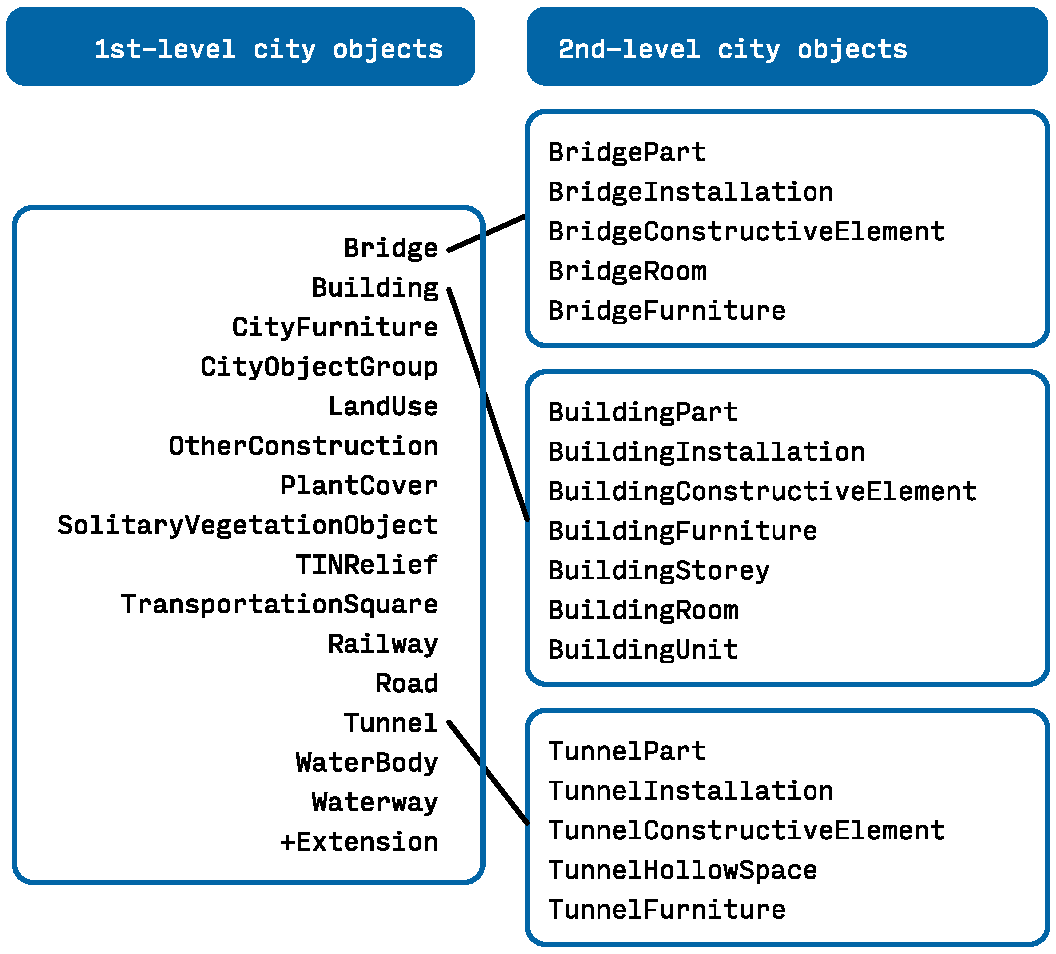
\includegraphics[width=0.7\linewidth]{figs/cityjson_co}
  \caption[The CityJSON classes]{The CityJSON classes (same name as CityGML classes) are divided into 1st and 2nd levels.}%
\label{fig:cityjson_co}
\end{figure}

%

As an example, for a \texttt{Building} containing 2 \texttt{BuildingPart}s, the 3 objects will be represented at the same level and linked by their \emph{IDs}.
\begin{lstlisting}
  "CityObjects": {
    "id-1": {
      "type": "Building",
      "attributes": {...},
      "children": ["id-2", "id-3"],
      "geometry": [{...}]
    },
    "id-2": {
      "type": "BuildingPart",
      "parents": ["id-1"],
      "geometry": [{...}]
      ...
    },
    "id-3": {
      "type": "BuildingPart",
      "parents": ["id-1"],
      "geometry": [{...}]
      ...
    }
  }
\end{lstlisting}

%

Each city object can have a \texttt{"parents"} and/or a \texttt{"children"} property, and this is how in the snippet the building \texttt{"id-1"} is linked to its 2 parts.
% We define 2nd-level city objects as having a \texttt{"parent"}.
The fact that a dictionary is used means that developers have direct access to the city objects through their IDs (and also in constant time if a hash map is used to implement the dictionary).

%

A city object can be of any of the types defined in Figure~\ref{fig:cityjson_co}, and each of them must have the same structure, and at a minimum contain a \texttt{"geometry"} property. 
If attributes are to be stored, they have to be in the \texttt{"attributes"} property.
This simplifies the work of the developer because there is a single point of entry for all geometries and attributes, unlike with XML-encoded CityGML\@.
\begin{lstlisting}
  {
    "type": "PlantCover",
    "attributes": {
      "averageHeight": 11.05,
      "colour": "green"
    },
    "geometry": [{...}]
  }
\end{lstlisting}


%%%
\subsection{Geometry}

CityJSON defines the same 3D geometric primitives used in CityGML, with the same restrictions for linearity/planarity.
\marginnote{ISO19107 geometries are used}
However, since they are rarely used in a 3D context, \emph{Point} and \emph{LineString} only have their Multi* counterparts; a single \emph{Point} is a \emph{MultiPoint} with only one object.
When a geometry is defined, it must contain a value for the LoD. 
In order to avoid ambiguities, we encourage the use of the TUDelft LoDs (see above), over the four standard CityGML ones.
City Object can have several LoDs, and thus CityJSON, as is the case for CityGML, allows us to store concurrently several LoDs for the same object.
\begin{lstlisting}
  {
    "type": "MultiSurface",
    "lod": 2.1,
    "boundaries": [
      [[0, 3, 2, 1]], [[4, 5, 6, 7]], [[0, 1, 5, 4]]
    ]
  }
\end{lstlisting}

It should be noticed that CityJSON uses a different approach from GML and CityGML-XML to store the $(x,y,z)$ coordinates of geometric primitives.
A geometric primitive does not list all the coordinates of its vertices, rather the coordinates of the vertices are stored in a separate array (the \texttt{"vertices"} property of the CityJSON object), and geometric primitives refer to the position of a vertex in that array.
\begin{lstlisting}
  "vertices": [
    [23234, 111009, 1392],
    [29456, 115134, 1007],
    [54508, 229995, 1961],
    ...
    [23134, 625134, 203]
  ]
\end{lstlisting}
The indexing mechanism of the format \emph{Wavefront OBJ}\marginnote{\faExternalLink\ \url{https://en.wikipedia.org/wiki/Wavefront_.obj_file}} is reused, because it has been used for many years, with success, in the computer graphics community.
This mechanism is modified so that the coordinates of the vertices of the geometries are represented as integer values (and not floats).
This is to reduce the size of a CityJSON object (and thus the size of files) and to ensure that only a fixed number of digits is stored for the coordinates of the geometries (eg to have millimetre precision).
This is achieved by using a simple \emph{quantization} method, 
\marginnote{\faExternalLink\ \url{https://www.cityjson.org/specs/\#transform-object}}
where the scale factor and the translation needed to obtain the original coordinates are stored.

There are several advantages to storing vertices once (instead of repeating them as in GML).
First, the files can be compressed: 3D vertices are often shared by several surfaces, and repeating them can be costly (especially if they are very precise, often sub-millimetre is used).
Second, this increases the topological relationships that are explicitly stored in the file, and several operations can be sped up and made more robust (\eg\ are two buildings adjacent?).
Third, it is very easy to convert to a representation listing all coordinates; the inverse is not true. 

%

The geometry is based on an enumeration of the vertices forming each ring of a surface, as follows.
A \texttt{"MultiSurface"} has an array containing surfaces, where each surface is modelled by an array of arrays, the first array being the exterior boundary of the surface, and the others the interior boundaries.
A \texttt{"Solid"} has an array of shells, the first array being the exterior shell of the solid, and the others being the interior shells; each shell has an array of surfaces, modelled in the exact same way as a \texttt{"MultiSurface"}.
Notice that unlike with GML and CityGML-XML, there is only one variation per geometry type, which (greatly) simplifies the life of developers.
\marginnote{Concrete examples of each geometric type are given at \faExternalLink\ \url{https://www.cityjson.org/dev/geom-arrays/}.}
\begin{lstlisting}
  {
    "type": "Solid",
    "lod": 2.2,
    "boundaries": [
      [ [[0, 3, 2, 1, 22]], [[4, 12, 123, 5, 6, 7]], [[0, 1, 5, 4]], [[1, 2, 6, 5]] ], 
      [ [[240, 243, 124]], [[244, 246, 724]], [[34, 414, 45]], [[111, 246, 5]] ] 
    ]
  }
\end{lstlisting}


%%%
\subsection{Appearance}

Both textures and materials are supported, and the same mechanisms as CityGML are used for these. 
The material is represented with the X3D specifications, as is the case for CityGML\@. 
\marginnote{\faExternalLink\ \url{https://en.wikipedia.org/wiki/X3D}}
For the texture, the COLLADA specifications are reused, as is the case for CityGML\@.
\marginnote{\faExternalLink\ \url{https://www.khronos.org/collada/}}


%%%
\subsection{Extension to the core model}

CityJSON also supports extensions to the core data model of CityGML for specific applications and use-cases.
They are simply called \emph{Extensions} and are defined as simple JSON files, and support the addition of new feature types, as well as the addition of new attributes for features and for datasets. 
See \url{https://www.cityjson.org/specs/#extensions} for more details.



%%%
\subsection{CityGML support}

CityJSON implements most of the data model, and all the CityGML modules have been mapped to CityJSON objects. 
However, for the sake of simplicity and efficiency, some modules and features have been omitted and/or simplified. 
If a module is supported, it does not mean that there is a 1-to-1 mapping between the classes and features in CityGML and CityJSON, but rather that it is possible to represent the same information, but in a different manner. 
CityJSON thus conforms to a subset of CityGML, although technically only XML-encoded CityGML files can be conformant to the specifications of CityGML\@.

%

The main features that are \underline{not} supported are:
\marginnote{full list at: \url{https://www.cityjson.org/citygml/v30/}}
\begin{itemize}
  \item Several CRSs in the same datasets. In CityJSON, all geometries in a given CityJSON object must use the same CRS\@. In CityGML, 3 adjacent buildings can all have different CRSs, and some of the geometries to represent the walls can be in yet another CRS (although admittedly it is seldom used!).
  \item Identifiers for low-level geometries. In CityGML most objects can have an ID (usually a \texttt{gml:id}). That is, not only can one building have an ID, but also each of the 3D primitives forming its geometry can have an ID\@. In CityJSON, only city objects and semantic surfaces can have IDs.
  \item Complex attributes have been simplified. For instance, several attributes in CityGML are derived from \texttt{gml:Measure} (like \texttt{bldg:mea\-su\-red\-Height}), and thus you cannot just store a value but also the unit of measurement. This is not represented in CityJSON directly, an Extension must be used. Also, generic attributes in CityGML cannot be mapped simply because in CityJSON you can add any attributes you like (inline with the JSON philosophy).
  \item Raster files for the relief. Only TINs are supported.
\end{itemize}



%%%
%
\section[Other formats]{Other formats for 3D city modelling}
% \begin{enumerate}
%   \item LandInfra
%   \item OBJ, OFF
%   \item glTF?
% \end{enumerate}

We describe briefly in this section a few formats and standards that are related to 3D city modelling and that are sometimes used in practice.
Those generally focus mostly on \emph{geometries}, but lack support for semantics and attributes (to a varying degree).
They are thus usually less suitable and less agile than the family of CityGML formats, that is they can be useful for a few use-cases.



%%%
\subsection{Standard computer graphics formats: OBJ, PLY, OFF, etc}

There exist several similar formats in computer graphics for storing and representing meshes (which are usually triangular meshes, but polygons can also be represented):

\textbf{OBJ (Wavefront Object)} is one of the most popular text-based formats in the 3D graphics community.
\marginnote{OBJ specifications: \url{http://paulbourke.net/dataformats/obj/}}
It has a simple structure where first the vertices are listed, and then each polygon is listed, as a list of references to the vertex ID (its position in the list of vertices).
The OBJ format can also encode colours and texture information, which are stored in a separate file (a~\texttt{.mtl} file, Material Template Library).
Attributes for specific polygons or groups of polygons is only possible by using the comments and grouping possibilities (as a hack), there are no standardised and documented ways to do so.

\textbf{OFF} is a simpler format: only polygons can be represented, optionally with their colours.
\marginnote{OFF specifications: \url{https://en.wikipedia.org/wiki/OFF_(file_format)}}

\textbf{PLY} is based on the same ideas for the geometries, and attributes can also be attached to vertices and polygons. (See the \emph{Computational modelling of terrains} book Appendix~A).

Notice that neither of these formats allow us to store an ISO19107 solid having inner shells and attributes/semantics for different parts/elements.


%%%
\subsection{glTF (GL Transmission Format)}
glTF\marginnote{glTF specifications: \url{https://www.khronos.org/gltf/}} is a JSON-based open 3D format by Khronos Group for the exchange of 3D models.
It also has a binary encoding for storing mesh geometry and animation data.
It provides compact representation of geometries, and small file sizes.

It is used for instance in CesiumJS\marginnote{CesiumJS: \url{https://cesium.com/cesiumjs/}} (which supports semantic 3D city models to some extents), and in other libraries like \emph{three.js}\marginnote{three.js: \url{https://threejs.org/}}.

% TODO: b3dm?


%%%
\subsection{LandInfra \& InfraGML}

LandInfra is a relatively new OGC open standard for land and infrastructure features, integrating concepts from IFC/BIM (see Chapter~\ref{chap:bim}) and CityGML\@.

It actually partially overlaps with CityGML: it contains the thematic classes `Building', `Road' and `Railway' (\texttt{Transportation} in CityGML), and `LandSurface' (\texttt{ReliefFeature} in CityGML). 
However, it has a more detailed representation for land and infrastructure features, \eg\ administrative units, ownership rights, spatial units for land use (land parcels and the legal spaces of buildings), surveying and representation, alignment for roads and railways, subsurface models for terrain, etc

InfraGML is the GML-based encoding of LandInfra, and the only one standardised.

LandInfra is a relatively young standard and at present it is difficult to identify any concrete examples of its usage in practice; the majority of citations about LandInfra describe the need to consider LandInfra in future work.


%%%
%
\section{Notes and comments}

The official specifications of CityGML are available at \url{https://www.opengeospatial.org/standards/citygml}.


\citep{Stadler07} first proposed and described the semantic and spatial decompositions of a city, and how keeping the two decomposition aligned has several advantages in practice.

\citet{Biljecki15a} describe and list 30 use-cases and 100 applications that make use of semantic 3D city models.

See \citet{Biljecki18} for an overview of the existing ADEs (for CityGML v2.0.0).

The official specifications of CityJSON are available at \url{https://www.cityjson.org/specs/}.

CityJSON specifications, examples datasets, tutorials, and software are available at \url{https://cityjson.org}.
\citet{Ledoux19} discuss in details the encoding and give concrete examples why they believe it is a superior encoding to XML for the CityGML data model; parts of this chapter was taken and adapted from that paper.

\citet{Helsinki19} describe the efforts and workflows used by the city of Helsinki to build both a textured mesh and semantic 3D city models of the city. 
Details about how the model is used in practice are also given.

\citet{Kumar19} describe the role and position of LandInfra with respect to CityGML and BIM/IFC\@.

For the description of LoD of other classes then buildings, see \citet{Kumar19} for terrains, \citet{Labetski18} for roads, and \citet{Ortega18} for trees.

%%%
%
\section{Exercises}

\begin{enumerate}
  \item It is stated that a given CityJSON file will be on average 6X compacter than an equivalent CityGML file. Explain why CityJSON files are compacter.
  \item Build manually a CityJSON file of a unit cube that represent a LoD2 building, and assign to its surfaces the correct semantics (roof, ground, façade). Add a few random attributes to the building. Make sure your file is valid by following that tutorial: \url{https://www.cityjson.org/tutorials/validation/}
  \item What would be the ``best'' format to store the textured mesh of Helsinki (in Figure~\ref{fig:mesh})?
\end{enumerate}
